\begin{figure}\centering
	\subfloat[]{
		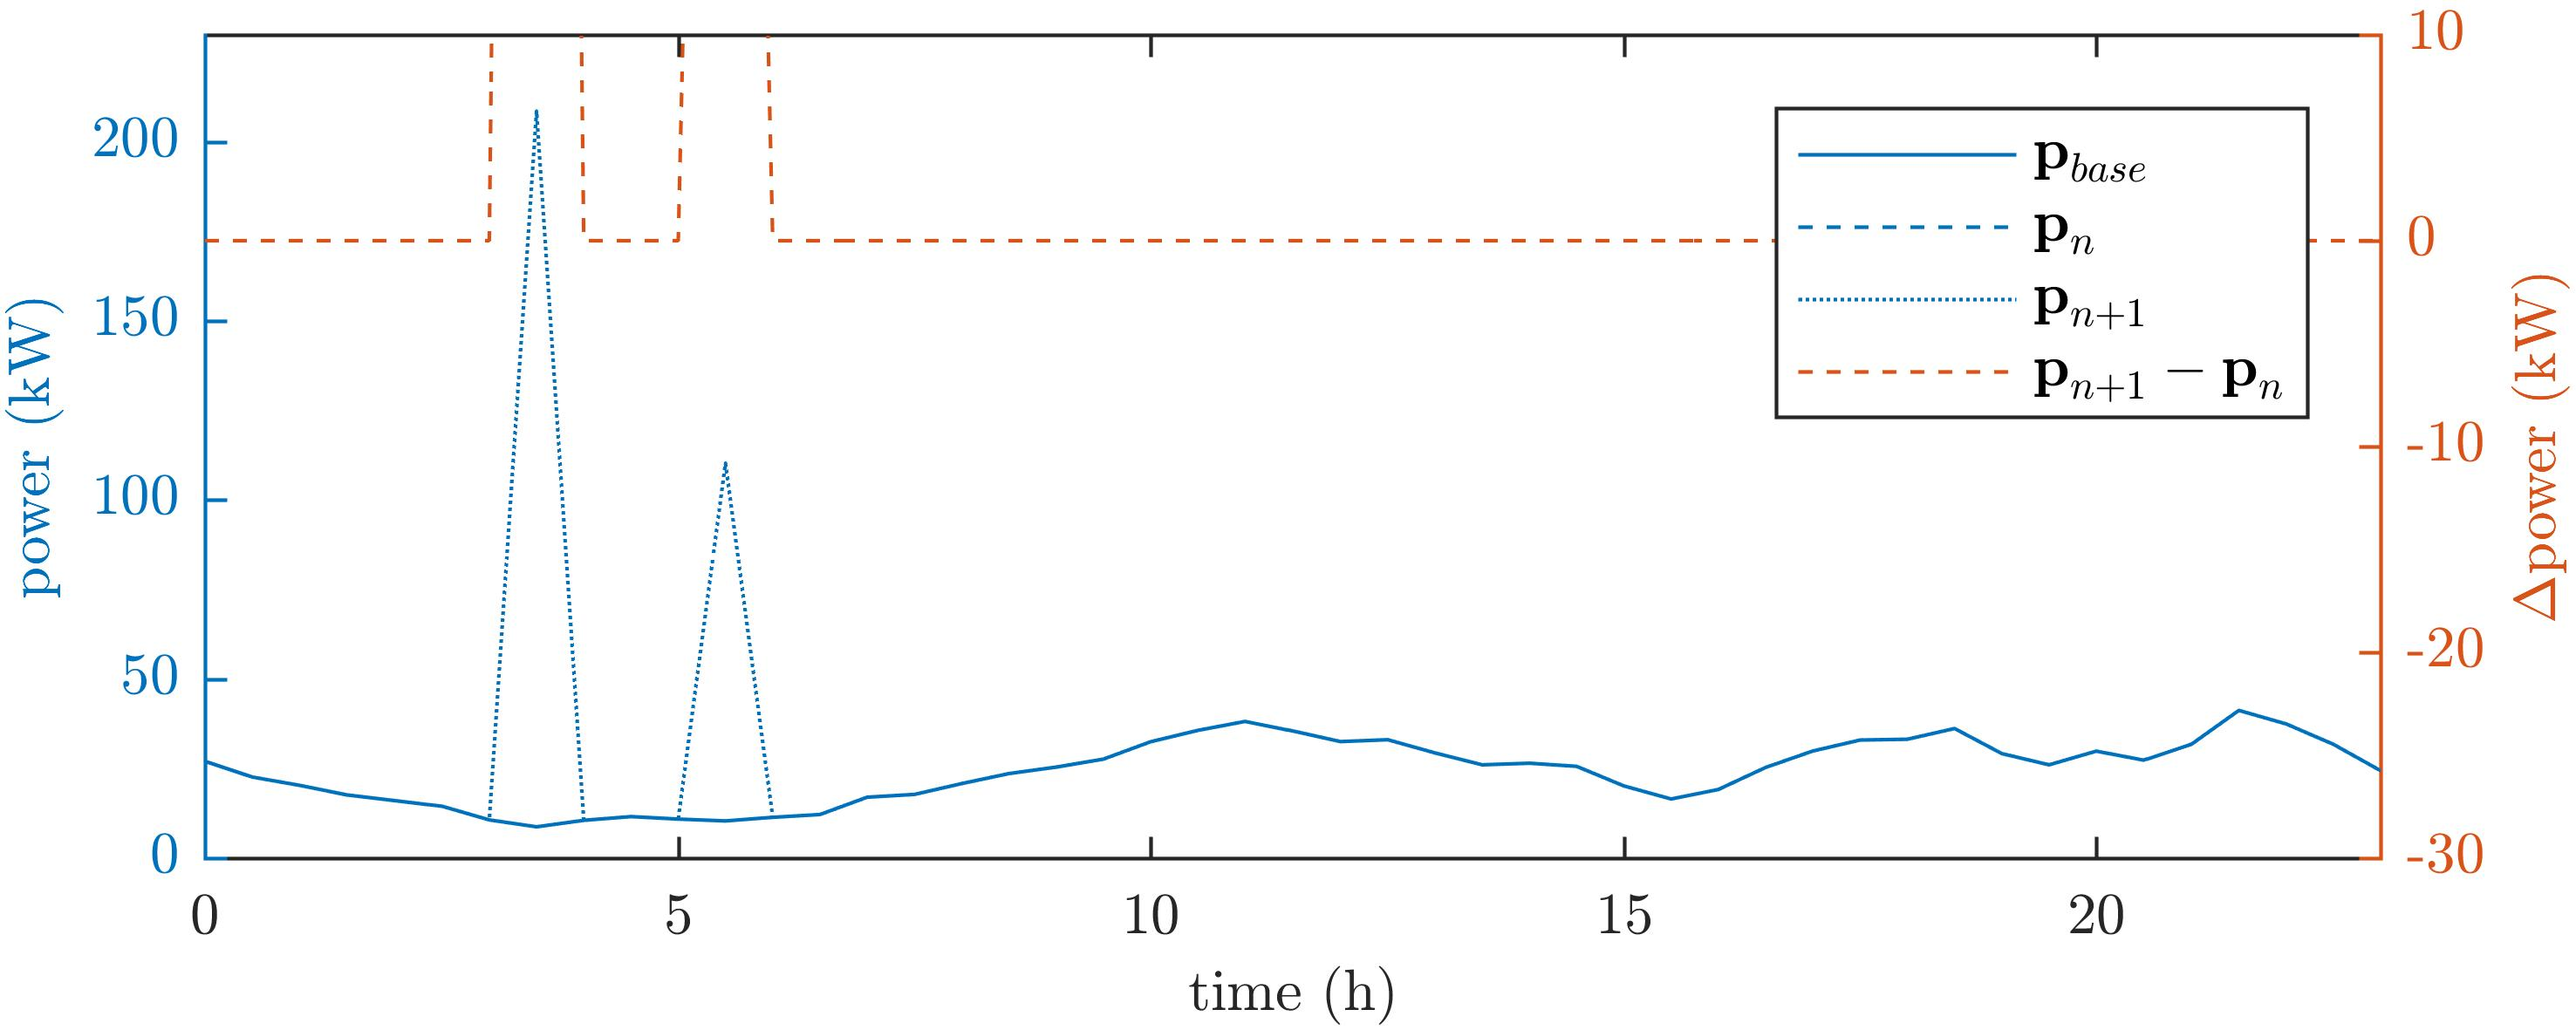
\includegraphics[height=4.5cm]{_chapter3/fig/time-series/ts-i0001}
		\label{ch3:subfig:time-series-1}
	}\\
	\subfloat[]{
		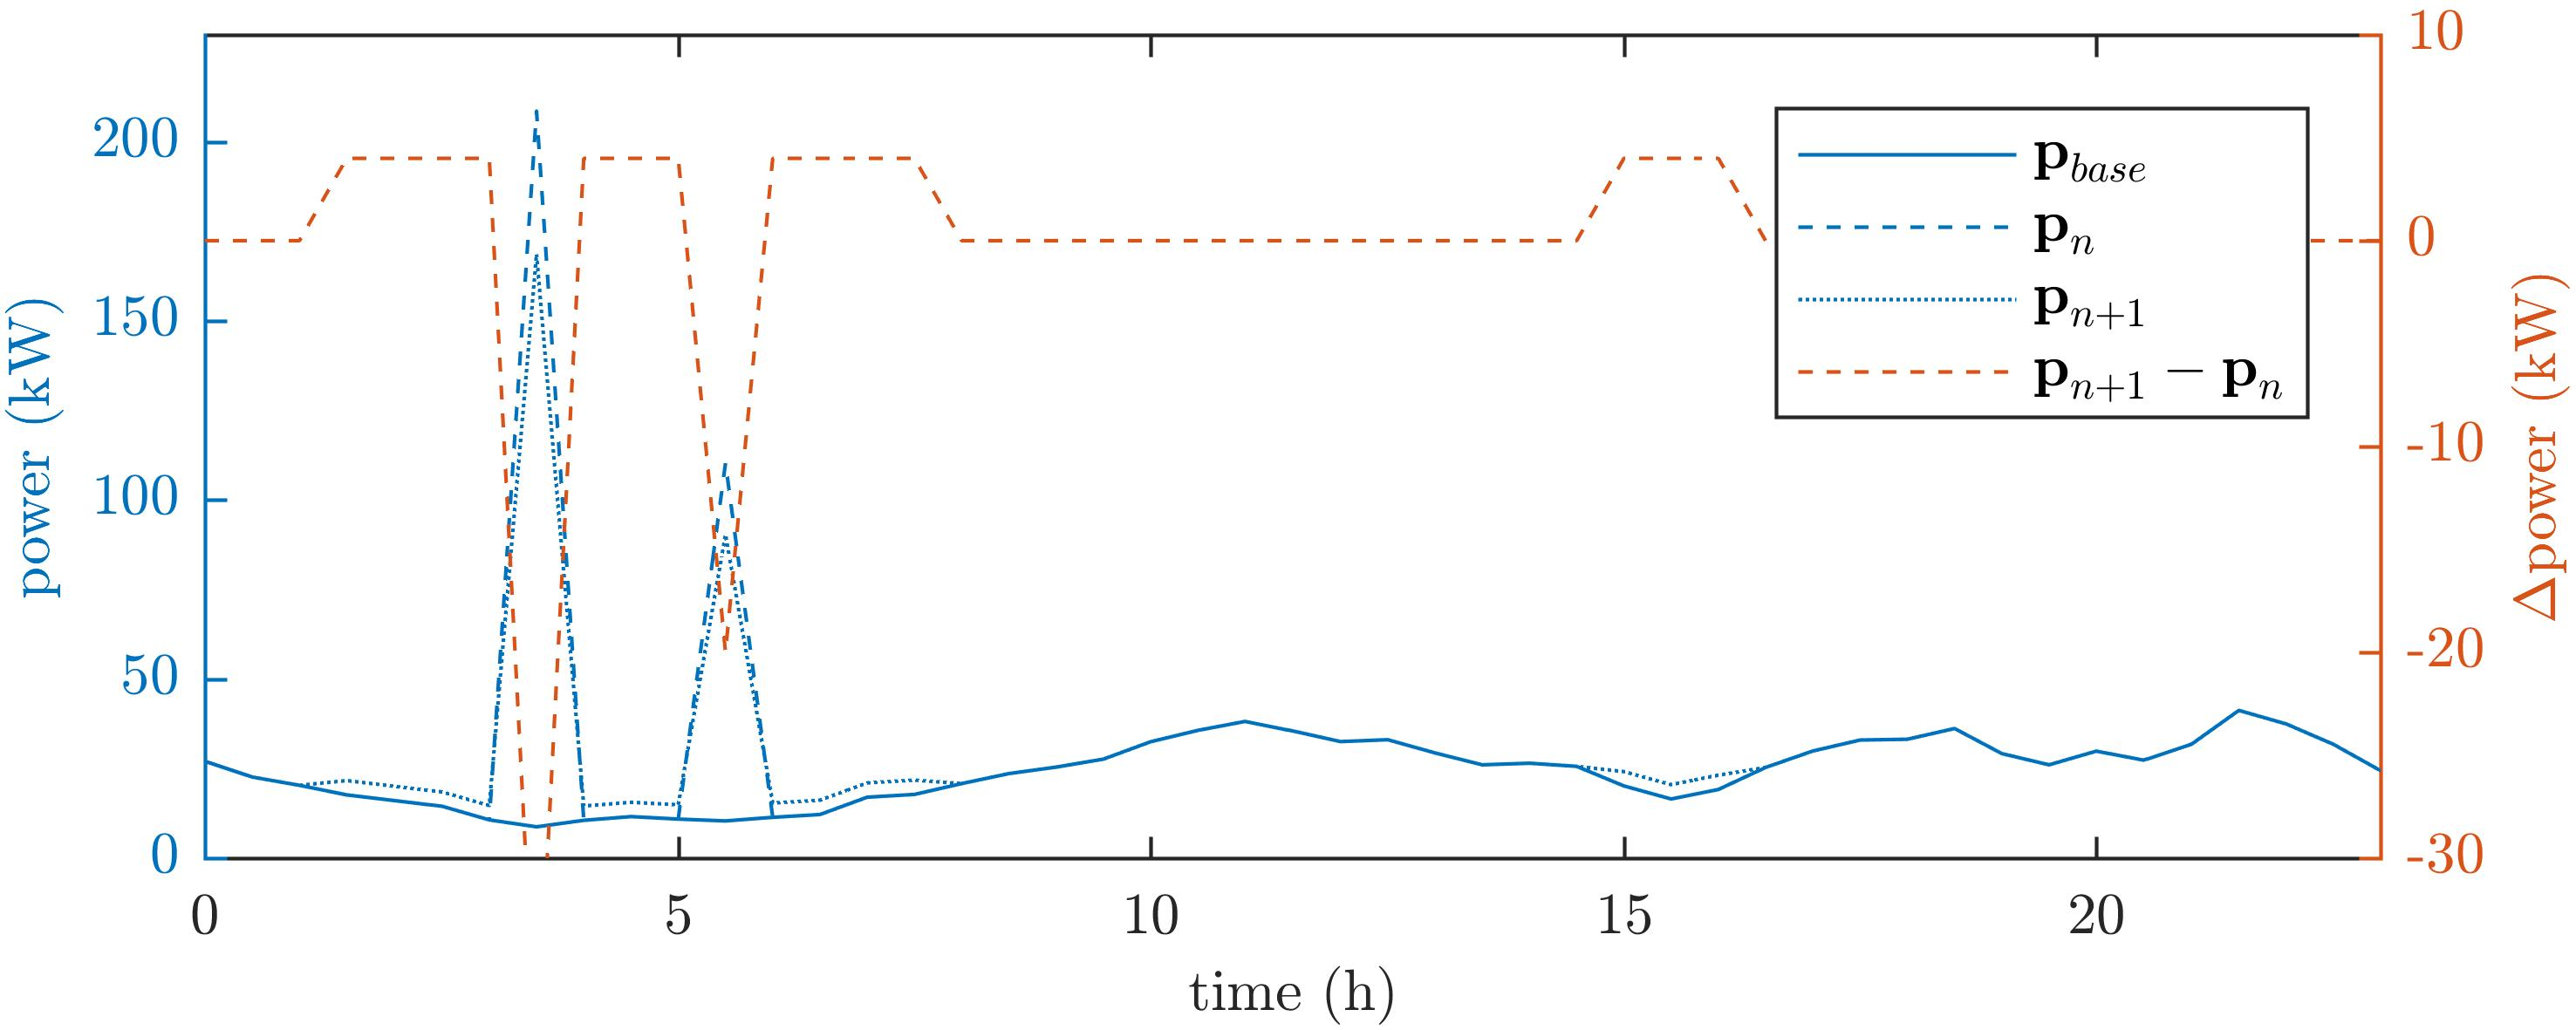
\includegraphics[height=4.5cm]{_chapter3/fig/time-series/ts-i0002}
		\label{ch3:subfig:time-series-2}
	}\\
	\subfloat[]{
		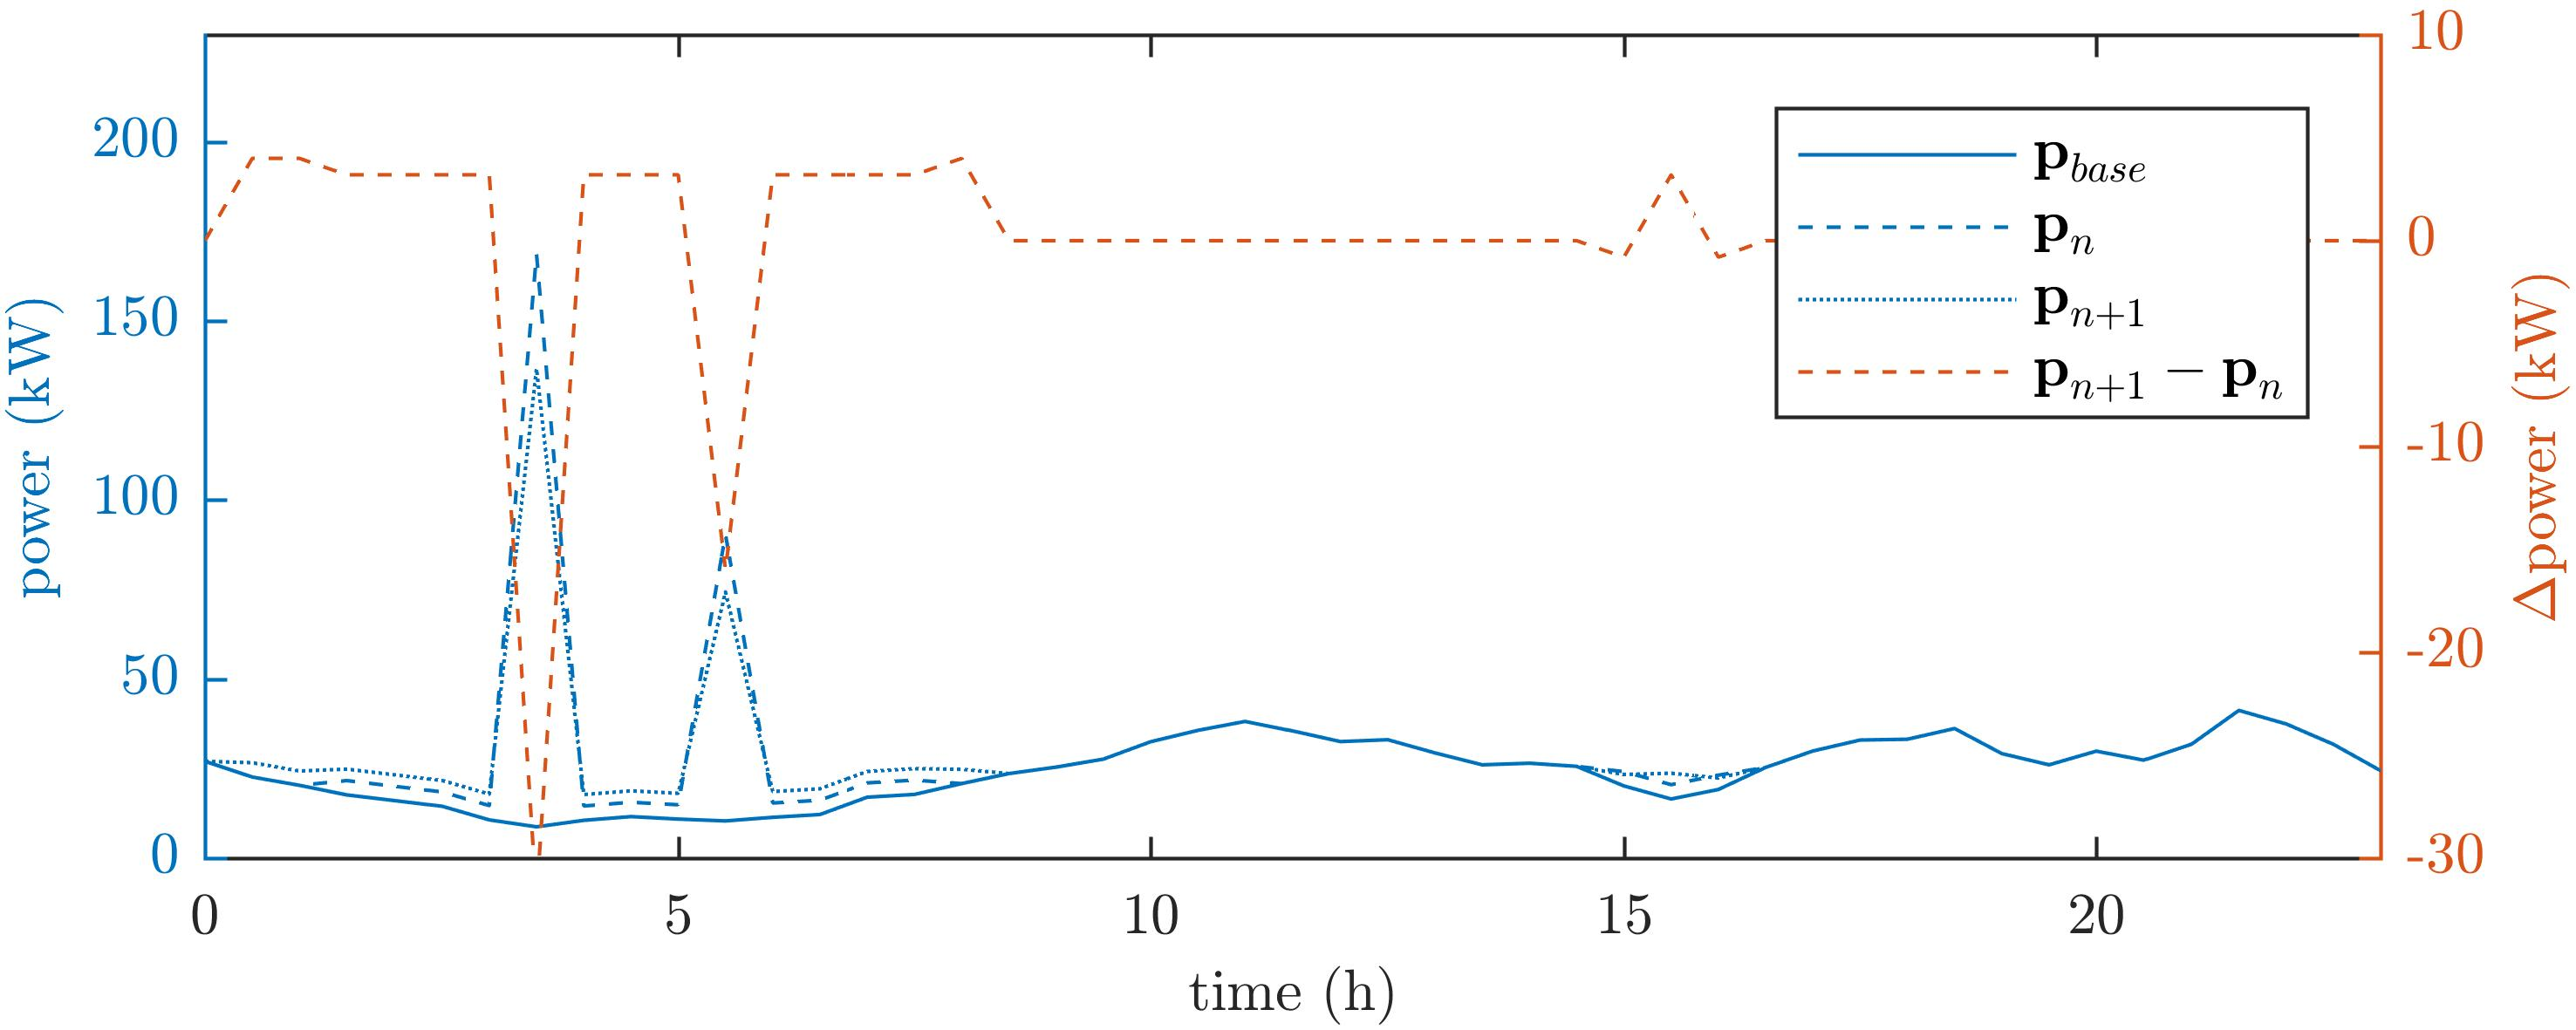
\includegraphics[height=4.5cm]{_chapter3/fig/time-series/ts-i0003}
		\label{ch3:subfig:time-series-3}
	}\\
	\subfloat[]{
		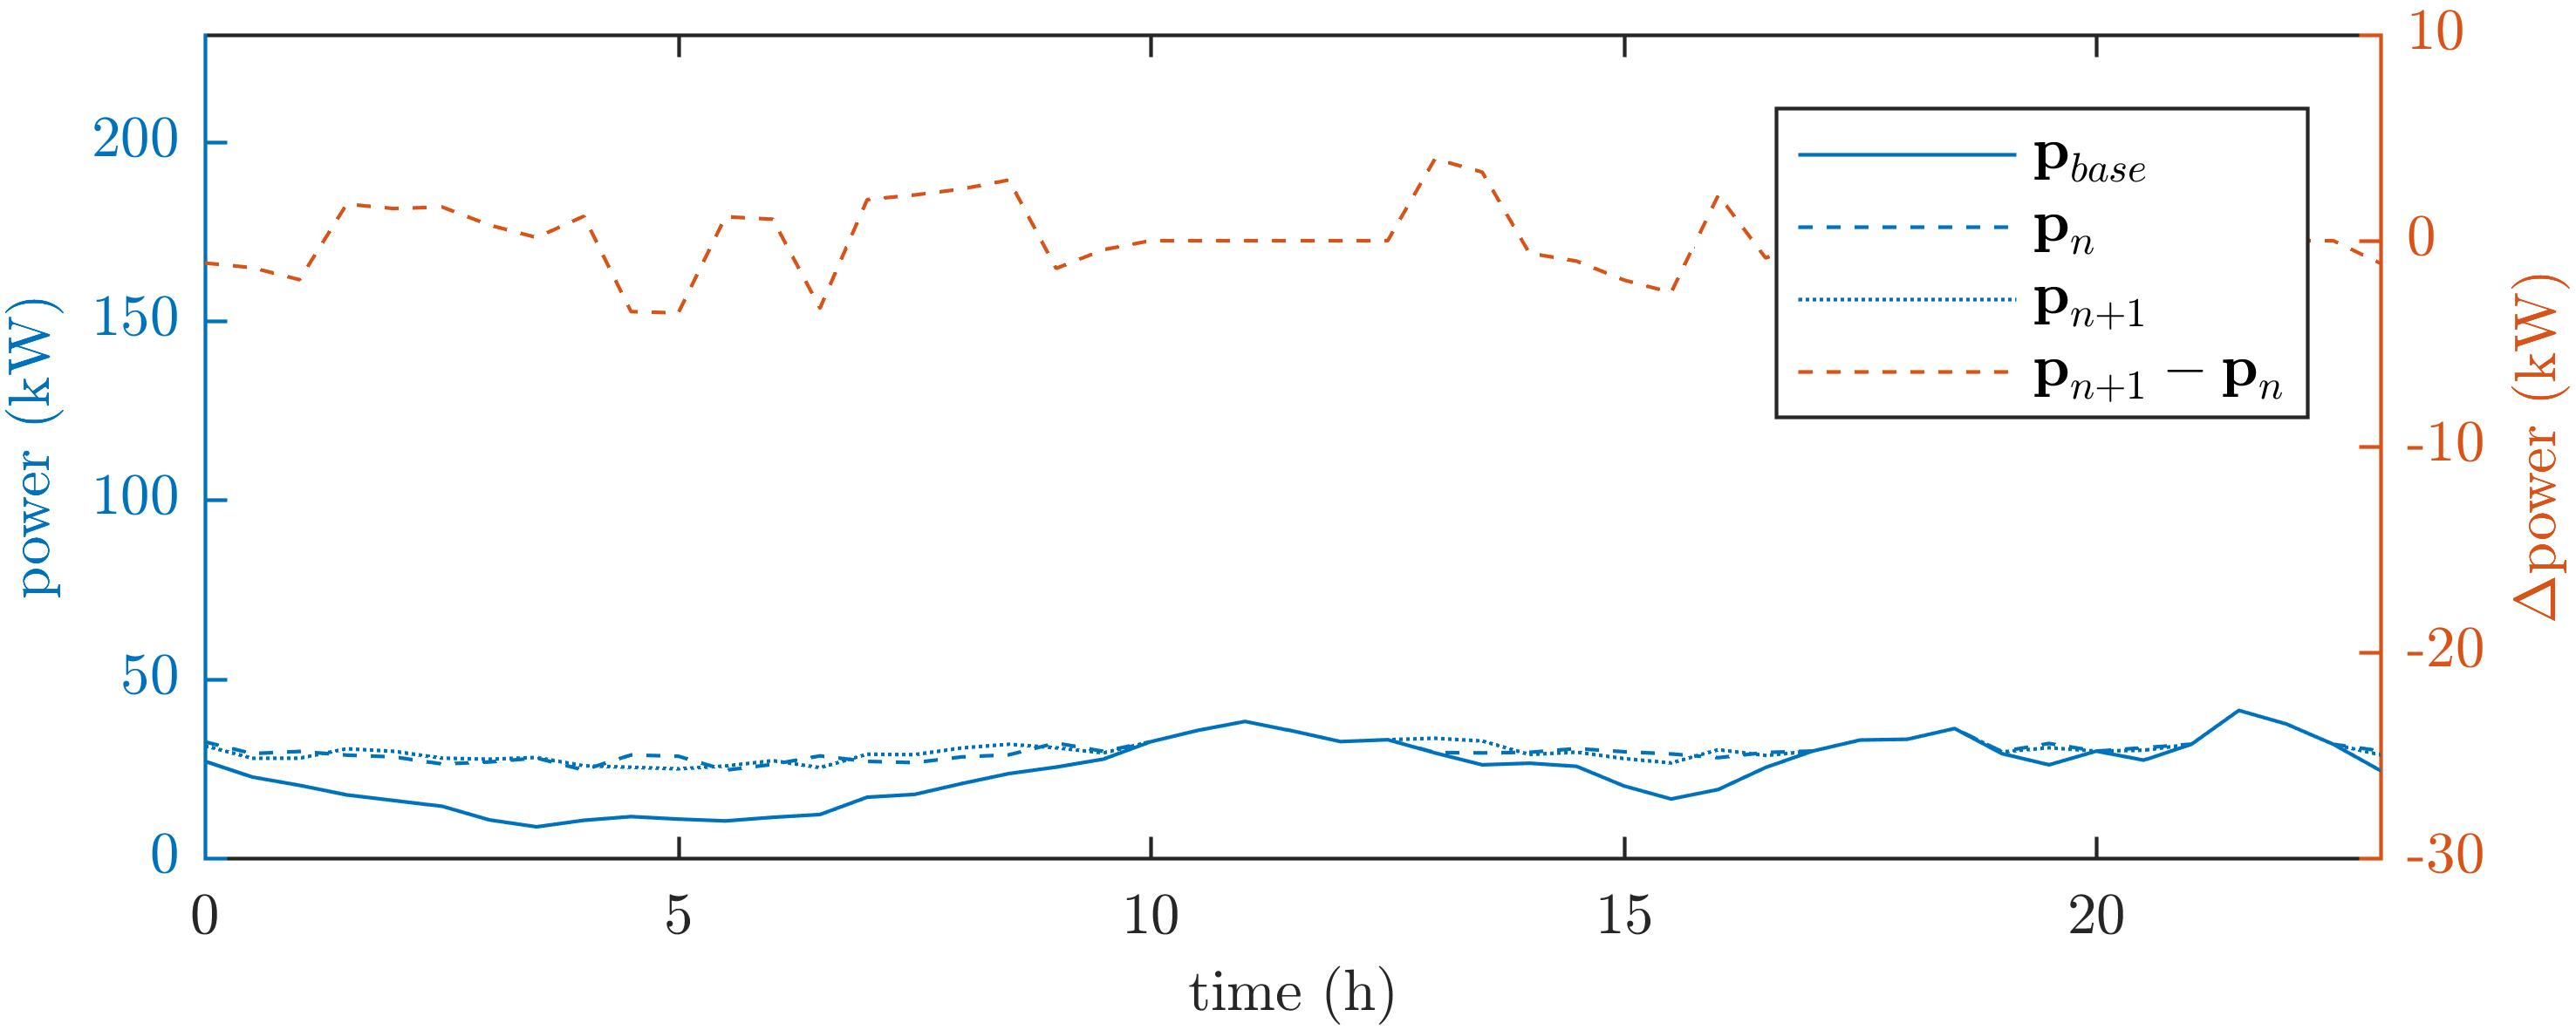
\includegraphics[height=4.5cm]{_chapter3/fig/time-series/ts-i0100}
		\label{ch3:subfig:time-series-last}
	}
\caption{Synchronised time series evolution for $\alpha=0.02$ and $\beta=0.20$, where (a) is at $n=1$, (b) is at $n=2$, (c) is at $n=3$, and (d) is at $n=N-1$.}
\label{ch3:fig:time-series}
\end{figure}